% siminos/presentations/kittens/catlatt.tex        pdflatex catlatt; biber catlatt
% $Author: predrag $ $Date: 2021-04-19 13:12:19 -0400 (Mon, 19 Apr 2021) $

                        \newif\ifboyscout\boyscouttrue          %% comments     %%
                        \newif\ifsubmission\submissionfalse     %% internal     %%
                        \newif\ifblog\blogfalse %% section shared with blogCats %%

\input ../../inputs/layoutBeamer
\usepackage[font=scriptsize, labelfont=bf]{caption}
\usepackage[
    backend=biber,  %bibtex,
    sorting=nyt,
    %refsection=chapter,
    %citereset=chapter,
    style=numeric, %alphabetic, % %style=authoryear,
    natbib=true,
    style=phys, % aps
    biblabel= brackets, % superscript, %
    articletitle=false, % true,  % false, % aps
    %chaptertitle=true,  % aip;  % false, % aps
    pageranges = true , % aip: the full range
             % = false, % aps: only the first page being printed
    sortlocale=en_US,
    firstinits=true,
    url=false, %true,  %
    doi=false, %true,
    eprint=false
]{biblatex}
\addbibresource{../../bibtex/siminos.bib}
\setbeamerfont{footnote}{size=\tiny}
%\input ../../inputs/def % no edits, always from dasbuch/book/inputs
\input defsKittens
\input ../../inputs/defsBeamer
\renewcommand{\Ssym}[1]{{\ensuremath{m_{#1}}}}    % Boris
% \newcommand{\Ssym}[1]{{\ensuremath{s_{#1}}}}  % ChaosBook
% \newcommand{\D}{\mathcal{D}}
% \newcommand{\gd}{\mathsf{g}}

\begin{document}
\title{
{\huge herding cats} %\catlatt}
    \\
{a chaotic field theory}
}
\author{P. Cvitanovi\'c}
\author[Cvitanovi\'c]
{
  \textcolor{green!50!black}{
  {Predrag~Cvitanovi\'c
   and
   Han Liang
%   \\
%  Matt Gudorf,
  }	%\inst{1}
  }
}
\institute
{
%  \inst{1}%
%\HREF{https://itsatcuny.org/calendar/chaos-and-quantum-field-theory}
%{ITS Symposium on Chaos and Quantum Field Theory}
 ChaosBook.org/overheads/spatiotemporal/kittens/   ~ notes
 \\
               Georgia Tech
 }
\date{September 27, 2020}

\begin{frame}
  \titlepage
\end{frame} %%%%%%%%%%%%%%%%%%%%%%%%%%%%%%%%%%%%%%%%%%%%%%


%\section[what this talk is about]
% {what this talk is about}
%
%\begin{frame}{overview}
%\begin{enumerate}
%              \item {\Large
%what this is about
%                  }\textcolor{gray}{\small
%%\\{\scriptsize \em
%%  (to skip the motivational blah blah: go to part \textcolor{red}{\ref{spacetimeFT}})
%%  }
%              \item
%chaos - a short course
%              \item
%\templatt
%              \item
%\catlatt
%              \item
%space is time
%              \item
%bye bye, dynamics
%                    }
%            \end{enumerate}
%\end{frame} %%%%%%%%%%%%%%%%%%%%%%%%%%%%%%%%%%%%%%%%%%%%%%

\section[\catlatt]
 {\catlatt}
\label{s:catLatt}

\begin{frame}{}
\begin{bartlett}{
I have said it thrice: \\
What I tell you three times is true.
        }
\bauthor{
Lewis Carrol,
{\em The Hunting of the Snark}
    }
\end{bartlett}
\vfill
\begin{enumerate}
              \item \textcolor{gray}{\small
%what this is about
%              \item
coin toss
              \item
kicked rotor
                  }
              \item {\Large
\catlatt
                  }\textcolor{gray}{\small
              \item
bye bye, dynamics
                    }
            \end{enumerate}
\end{frame} %%%%%%%%%%%%%%%%%%%%%%%%%%%%%%%%%%%%%%%%%%%%%%

\begin{frame}{spatiotemporally infinite `\catlatt'}
%\begin{center}
%\hfill
\includegraphics[width=0.55\textwidth]{spatiotempCat}
\hfill
\includegraphics[width=0.55\textwidth]{DawnBishopCats}
%\end{center}
\end{frame} %%%%%%%%%%%%%%%%%%%%%%%%%%%%%%%%%%%%%%%%%%%%%%


\begin{frame}{herding cats in $d$ spacetime dimensions}
start with
\begin{block}{a cat at each lattice site}
\bigskip

talk to neighbors
\medskip

spacetime $d$\dmn\
~~~~~~~ {\color{blue}\Large \catlatt}
\end{block}

\vfill

\begin{itemize}
  \item {\scriptsize Hamiltonian formulation is awkward, fuggedaboutit!}
  \item Lagrangian formulation is elegant
\end{itemize}
\end{frame} %%%%%%%%%%%%%%%%%%%%%%%%%%%%%%%%%%%%%%%%%%%%%%

\begin{frame}{\catlatt}
consider
a 1 {\color{blue}spatial} dimension lattice, with field
$\ssp_{nt}$ \\
(the angle of a kicked
rotor ``particle'' at instant $t$, at site $n$)
\begin{block}{require}
\begin{itemize}
\item  each site couples to
its nearest neighbors $\ssp_{n\pm1,t}$
\item  invariance under
spatial translations
\item  invariance under spatial reflections
\item  invariance under the space-time exchange
\end{itemize}
\end{block}

\bigskip

Gutkin \& Osipov\footfullcite{GutOsi15} obtain
\begin{block}{2\dmn\ coupled cat map lattice}
\[
\ssp_{n,t+1} + \ssp_{n,t-1} - 2s \, \ssp_{n t} + \ssp_{n+1,t} + \ssp_{n-1, t}
     =-\Ssym{n t}
\] %\ee{eq:CatMapNewton2}
\end{block}
\end{frame} %%%%%%%%%%%%%%%%%%%%%%%%%%%%%%%%%%%%%%%%%%%%%%

\begin{frame}{\catlatt\ : a strong coupling field theory}
symmetries : translations $\circ$ time-reversal $\circ$ spatial reflections

\bigskip

\begin{block}{the key assumption}
\begin{itemize}
\item  invariance under the space-time exchange
\end{itemize}
\end{block}
\bigskip

{\color{red}not} a traditional \\
{\color{blue}spatially
weakly coupled} lattice model\footfullcite{BunSin88}
\bigskip
%assuming that coupling strengths along the time and space directions are
%the same makes \catlatt\ a maximally strongly coupled field theory
%
%
%
%in contrast to the usual weak-coupling lattice models
\vfill

\begin{itemize}
  \item \catlatt\ is a Euclidean field theory
%  \item in Lagrangian formulation
\end{itemize}
\end{frame} %%%%%%%%%%%%%%%%%%%%%%%%%%%%%%%%%%%%%%%%%%%%%%

\begin{frame}{herding cats : a discrete Euclidean space-time field theory}
write the spatial-temporal differences as discrete derivatives
\begin{block}{Laplacian in %$d=1$ and
              $d=2$ dimensions}
%\(
%\Box\,\ssp_t \;\;\,=\, \ssp_{t+1} - 2\ssp_{t} + \ssp_{t-1}
%\)\\
\(
\Box\,\ssp_{nt} \,=\, \ssp_{n,t+1} + \ssp_{n,t-1}
- 4 \, \ssp_{nt} + \ssp_{n+1,t} + \ssp_{n-1, t}
\)\\
~~~~{\scriptsize subtract 2\dmn\ coupled cat map lattice equation}\\
\(
-\Ssym{n t}
 =
\ssp_{n,t+1} + \ssp_{n,t-1} - 2s \, \ssp_{n t} + \ssp_{n+1,t} + \ssp_{n-1, t}
\) %\ee{eq:CatMapNewton2}
\end{block}

\bigskip

{\color{blue}cat herd} is thus governed by the law of
\begin{block}{$d$\dmn\ \catlatt}
\[
 (-\Box + {\mu}^2)\,\ssp_{z} = \m_z
\,, \qquad
{\mu}^2= d(s-2)
\] %\ee{LinearConn}

\medskip

\end{block}

\bigskip

where
\(
  \ssp_{z} \in [0,1)
    \,, \quad
  \Ssym{z} \in \A
    \mbox{  and  }
  z\in \integers^{d}
\) = integer lattice
\end{frame} %%%%%%%%%%%%%%%%%%%%%%%%%%%%%%%%%%%%%%%%%%%%%%

\begin{frame}{discretized linear PDE}
\begin{block}{$d$\dmn\ \catlatt}
{\Large
\[
 (-\Box + {\mu}^2)\,\ssp_{z} = \m_z
\] %\ee{LinearConn}
}
\end{block}

\bigskip

is linear and known as
\begin{itemize}
\item {\color{blue}tight-binding} model or {\color{blue}Helmholtz} equation \\
if stretching is weak, $s<2$ \\
 $[$oscillatory sine, cosine solutions]
\item
Euclidean {\color{blue}Klein-Gordon} or (damped {\color{blue}Poisson})\\
if stretching is strong, $s>2$ \\
 $[$hyperbolic sinches, coshes, `{\color{blue}mass}' ${\mu}^2=d(s-2)$]
\end{itemize}
\medskip

nonlinearity is hidden in the `sources'
\[
  \Ssym{z} \in \A
    \mbox{  at lattice site  }
  z\in \integers^{d}
\]
\end{frame} %%%%%%%%%%%%%%%%%%%%%%%%%%%%%%%%%%%%%%%%%%%%%%

\begin{frame}{spring mattress vs field of rotors}
\begin{center}
            \begin{minipage}[c]{0.40\textwidth}\begin{center}
traditional field theory
\bigskip

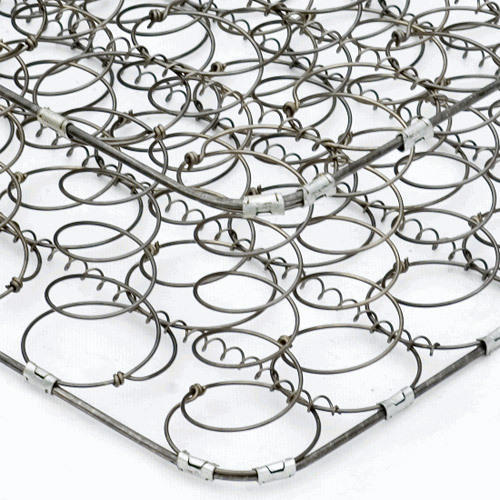
\includegraphics[width=0.85\textwidth]{mattressSpring}\\
{\color{blue}Helmholtz}
            \end{center}\end{minipage}
            \hspace{2ex}
            \begin{minipage}[c]{0.46\textwidth}\begin{center}
chaotic field theory\\
\bigskip
\bigskip
\bigskip

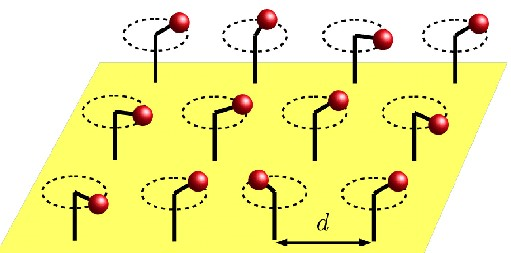
\includegraphics[width=1.0\textwidth]{flagellum1}\\
\bigskip

damped {\color{blue}Poisson}
            \end{center}\end{minipage}
\end{center}
\end{frame} %%%%%%%%%%%%%%%%%%%%%%%%%%%%%%%%%%%%%%%%%%%%%%

\begin{frame}{the simplest of all `turbulent' field theories ! }
\catlatt
\[
 (-\Box + {\mu}^2)\,\ssp_{z} = \m_z
\] %\ee{LinearConn}
\bigskip
\hfill can be solved completely (?) and analytically (!)

\bigskip
\bigskip

assign to each site $z$ a
letter \Ssym{z}\ from the alphabet $\A$.

\medskip

a particular fixed set
of letters  \Ssym{z}\ (a symbol \brick)
\[
\Mm= \{\Ssym{z}\} % \in \A \,,\; z\in \integers^d \}
 = \{\Ssym{n_1 n_2 \cdots n_d}\}
\,,
\]
is a complete specification of  \\
the corresponding lattice state $\Xx$
\bigskip

{\color{blue}\footnotesize
from now on work in $d=2$ dimensions, `stretching parameter'
$s=5/2$
}
\end{frame} %%%%%%%%%%%%%%%%%%%%%%%%%%%%%%%%%%%%%%%%%%%%%%

\begin{frame}{think globally, act locally}
solving the \catlatt\ equation
\[
\jMorb\Xx= -\Mm
\,,
\]
with
the $[\cl{}\!\times\!\cl{}]$ matrix ~~~~~
\(
\jMorb = \sum_{j=1}^{2}\left(\hopMat_j-{s}\unit+\hopMat_{j}^{-1}\right)
\) %{tempBernFix}
\medskip

can be viewed as a search for zeros of the function
\beq
F[\Xx] = \jMorb\Xx+\Mm = 0
\ee{tempFixPoint}
where the entire {\color{blue}global lattice state} ${\Xx}_{\Mm}$ is
\medskip

a single {\color{blue}fixed point}
${\Xx}_{\Mm}=\{\ssp_z\}$

\hfill
in the \speriod{}\period{}\dmn\ unit hyper-cube $\Xx\in[0,1)^{\speriod{}\period{}}$
\medskip

$\speriod{}$ is the `spatial',
$\period{}$ the `temporal' lattice period
\end{frame} %%%%%%%%%%%%%%%%%%%%%%%%%%%%%%%%%%%%%%%%%%%%%%

\begin{frame}{think globally, act locally}
    \begin{center}
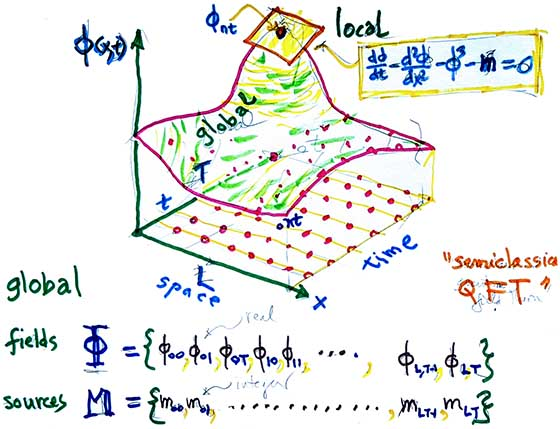
\includegraphics[width=0.85\textwidth]{globalLocal}
    \end{center}
for each symbol array \Mm, a periodic lattice state $\Xx_\Mm$
\end{frame} %%%%%%%%%%%%%%%%%%%%%%%%%%%%%%%%%%%%%%%%%%%%%%

\begin{frame}{next, enumerate all periodic spacetime tilings of the  integer lattice}
each tile : 2\dmn\ {(sub)lattice}, an infinite array of points
\beq
\Lambda = \{n_1 {\bf a}_1 + n_2 {\bf a}_2\,|\,n_i \in \mathbb{Z}\}
\ee{2DBravaisLattice}
with the defining tile spanned by a pair of basis vectors
$\mathbf{a}_{1},\mathbf{a}_{2}$

    \begin{block}{example : four tiles of area 10}
\hfill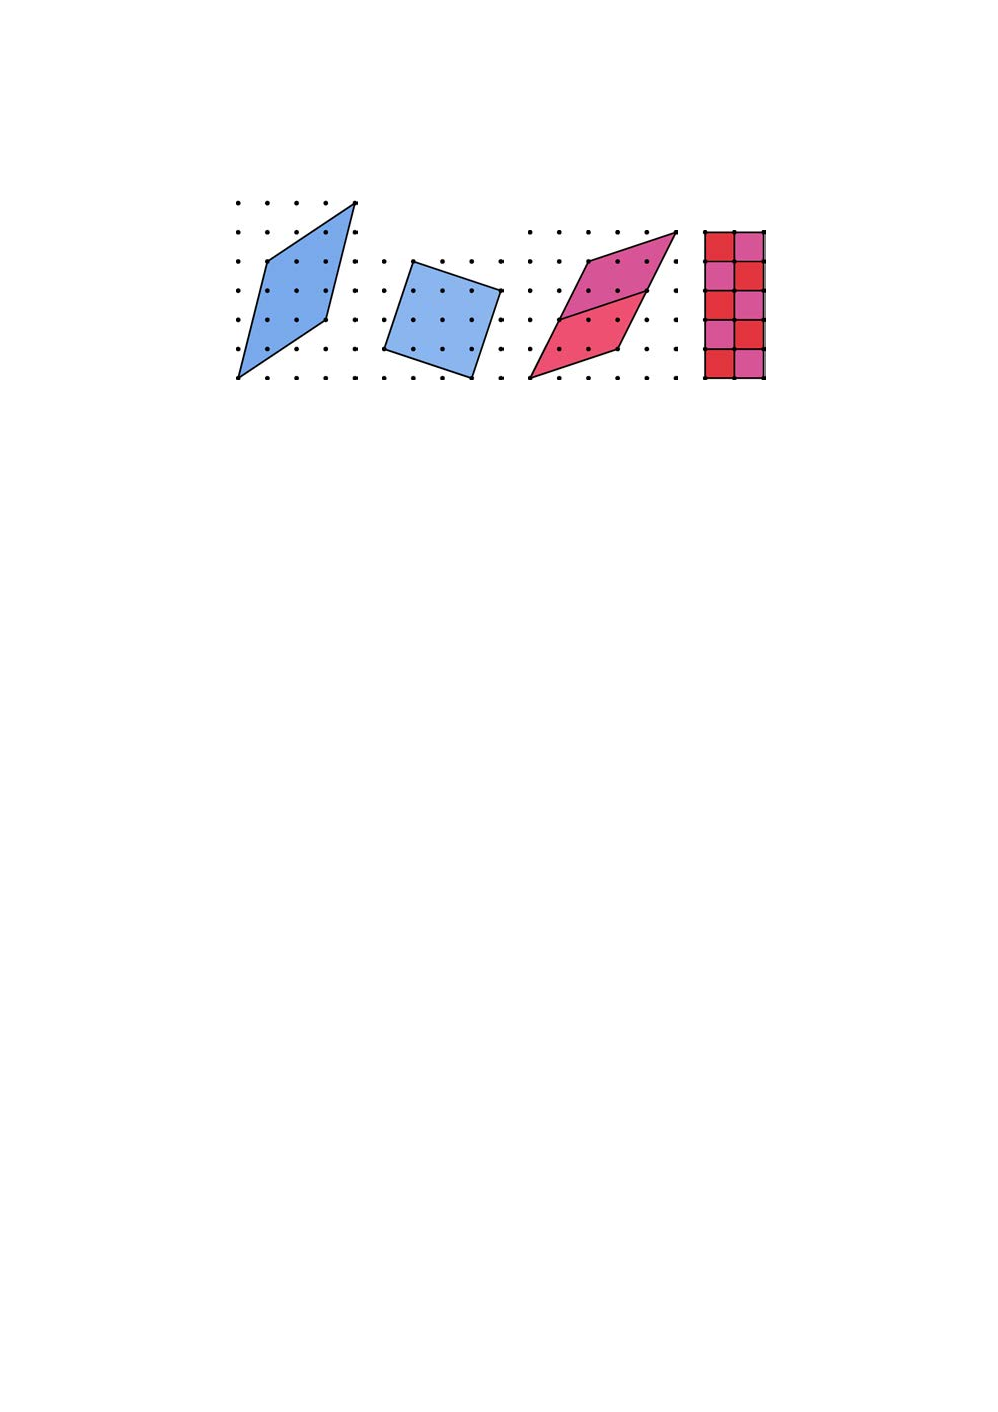
\includegraphics[width=0.7\textwidth]{Holmin15-Fig1}
    \end{block}
\bigskip
The two blue tiles appear
`prime', \ie, not
tiled by smaller tiles.
\textcolor{red}{False!}~~~~~
all four big tiles can tilled by smaller ones.
%          }\label{Holmin15-Fig1}

\vfill\hfill
{\Huge \textcolor{red}{tricky!}}
\end{frame} %%%%%%%%%%%%%%%%%%%%%%%%%%%%%%%%%%%%%%%%%%%%%%

\begin{frame}{$2$\dmn\ lattice tilings}
2\dmn\ {\color{blue}\emph{lattice}} is
defined by a $[2\times2]$ {\color{blue}\fundPip} matrix whose columns are basis vectors
\[
\mathbf{A} =
\left[ \mathbf{a}_{1} \mathbf{a}_{2} \right]
 =
\left[
\begin{array}{cc}
\speriod{} & \tilt{} \\
0 & \period{}
\end{array}
\right]
\,,
\]
$\speriod{}$, $\period{}$ : spatial, temporal
lattice periods\\
`tilt'  $0\leq\tilt{}<\speriod{}$ imposes the
{\color{blue}\emph{relative-periodic}}\\
(\emph{`helical'}, \emph{`toroidal'},
\emph{`twisted'}, \emph{`screw'},  $\cdots$
) {\bcs}

    \begin{block}{example : $[3\!\times\!2]_1$ tile}
\begin{center}
            \begin{minipage}[c]{0.32\textwidth}\begin{center}
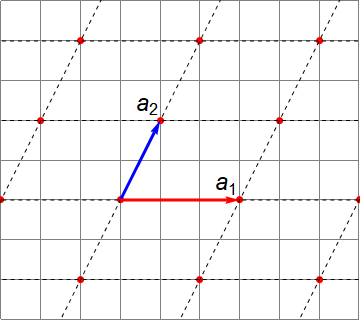
\includegraphics[width=1.0\textwidth]{HLBravaisLattice}
            \end{center}\end{minipage}
            \hspace{2ex}
            \begin{minipage}[c]{0.46\textwidth}
basis vectors
\\

${\bf a}_1=\left(
 \begin{array}{c}
 3\\
 0
 \end{array}
 \right)$,
${\bf a}_2=\left(
 \begin{array}{c}
 1\\
 2
 \end{array}
 \right)$
            \end{minipage}


\end{center}
    \end{block}
\end{frame} %%%%%%%%%%%%%%%%%%%%%%%%%%%%%%%%%%%%%%%%%%%%%%

\begin{frame}{exponentially many periodic lattice states in Felinestan}
\begin{center}
%%%%%%%%%%%%%%%%%%%%%%%%%%%%%%%%%%%%%%%%%%%%%%%%%%%%%%%%%%%%%
% HL 2020-06-09 siminos/figSrc/han/Mathematica/ColorBlock.nb
%\begin{figure}\begin{center}
            \begin{minipage}[c]{0.25\textwidth}\begin{center}
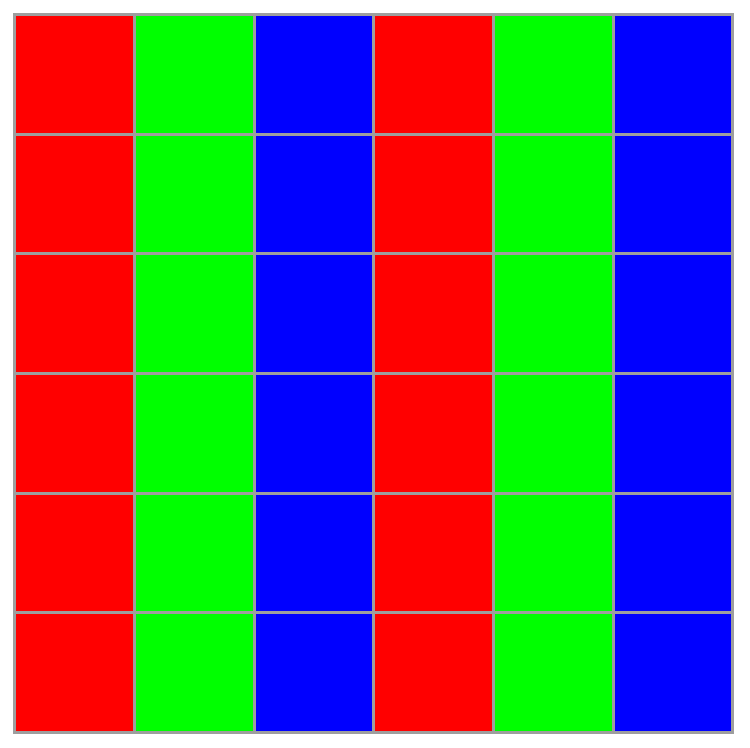
\includegraphics[width=1.0\textwidth]{HL310Block}\\$\BravCell{3}{1}{0}$ %(a)
            \end{center}\end{minipage}
            \hskip 4ex
            \begin{minipage}[c]{0.25\textwidth}\begin{center}
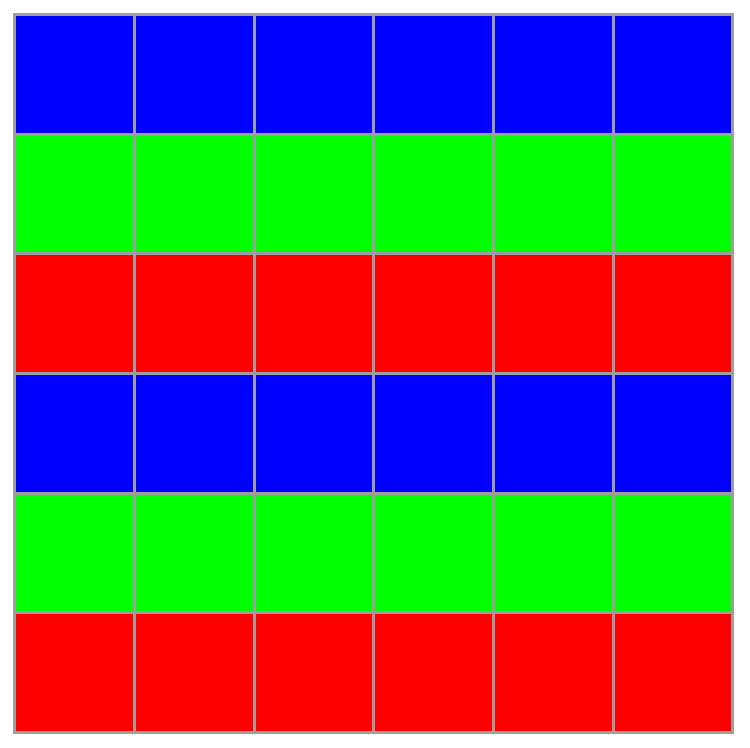
\includegraphics[width=1.0\textwidth]{HL130Block}\\$\BravCell{1}{3}{0}$ %(b)
            \end{center}\end{minipage}
            \hskip 4ex
            \begin{minipage}[c]{0.25\textwidth}\begin{center}
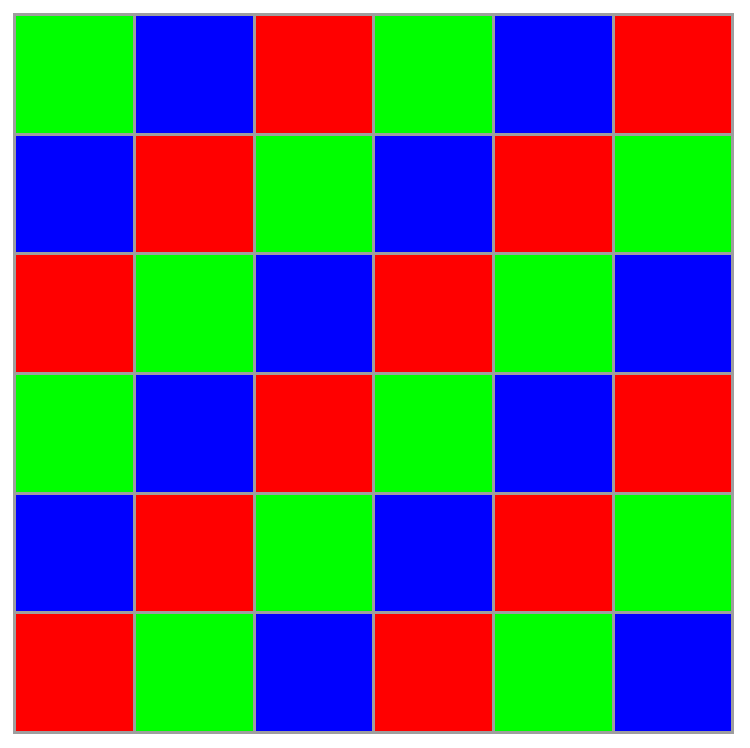
\includegraphics[width=1.0\textwidth]{HL311Block}\\$\BravCell{3}{1}{1}$ %(c)
            \end{center}\end{minipage}
%\end{center}
%  \caption{\label{fig:SpecialBravaisLatt}
%Examples of $\LTS{}{}{}$ periodic \brick s
%together with their \spt\ Bravais lattice tilings \refeq{2DBravaisLattice}.
%(a)
%$\BravCell{3}{1}{0}$, basis vectors
%$\mathbf{a}_1=\{3,0\}$ and $\mathbf{a}_2=\{0,1\}$;
%(b)
%$\BravCell{1}{3}{0}$, basis vectors
%$\mathbf{a}_1=\{1,0\}$ and $\mathbf{a}_2=\{0,3\}$;
%(c)
%$\BravCell{3}{1}{1}$, basis vectors
%$\mathbf{a}_1=\{3,0\}$ and $\mathbf{a}_2=\{1,1\}$;
%}
%%%%%%%%%%%%%%%%%%%%%%%%%%%%%%%%%%%%%%%%%%%%%%%%%%%%%%%%%%%%%
% HL 2020-06-09 siminos/figSrc/han/Mathematica/ColorBlock.nb
%\begin{figure}\begin{center}
            \begin{minipage}[c]{0.25\textwidth}\begin{center}
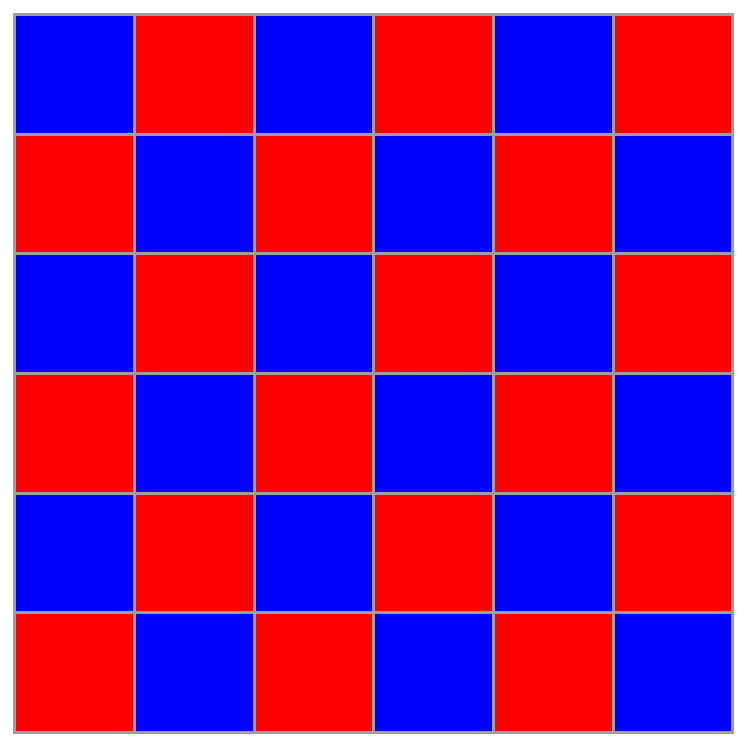
\includegraphics[width=1.0\textwidth]{HL211Block}\\$\BravCell{2}{1}{1}$ %(a)
            \end{center}\end{minipage}
            \hskip 4ex
            \begin{minipage}[c]{0.25\textwidth}\begin{center}
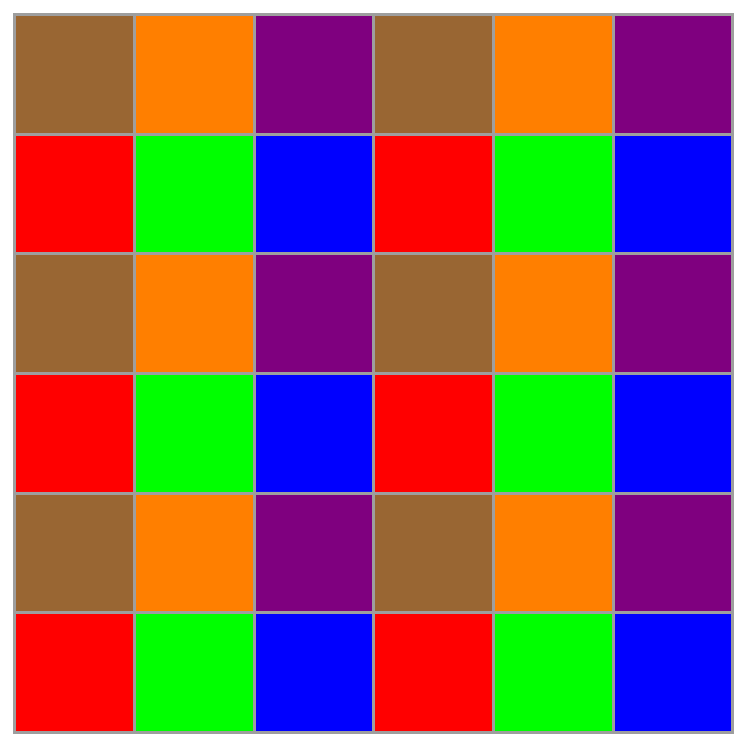
\includegraphics[width=1.0\textwidth]{HL320Block}\\$\BravCell{3}{2}{0}$ %(b)
            \end{center}\end{minipage}
            \hskip 4ex
            \begin{minipage}[c]{0.25\textwidth}\begin{center}
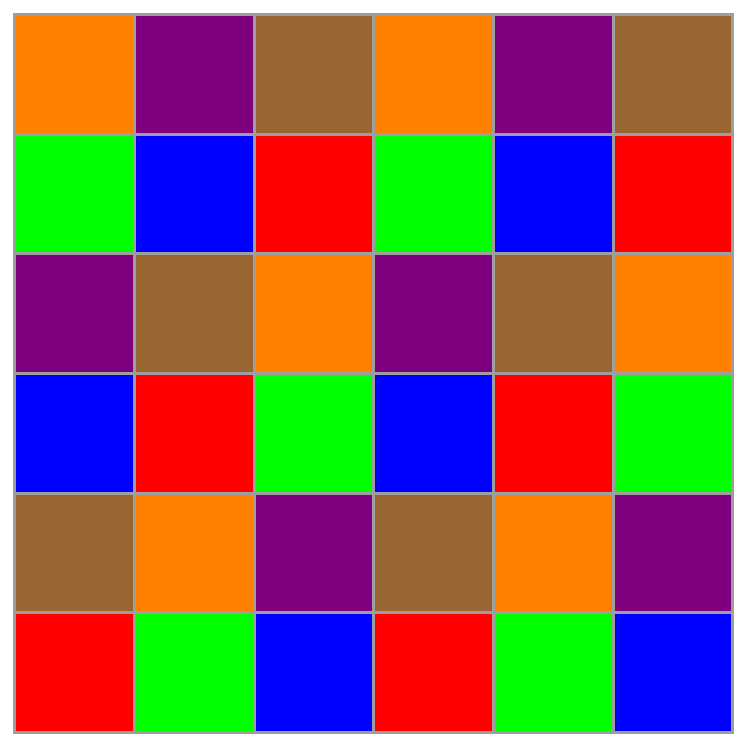
\includegraphics[width=1.0\textwidth]{HL321Block}\\$\BravCell{3}{2}{1}$ %(c)
            \end{center}\end{minipage}
%\end{center}
%  \caption{\label{fig:3x2rpo}
%Examples of $\LTS{}{}{}$ periodic \brick s
%together with their \spt\ Bravais lattice tilings \refeq{2DBravaisLattice}.
%(a)
%$\BravCell{2}{1}{1}$, basis vectors
%$\mathbf{a}_1=\{2,0\}$ and $\mathbf{a}_2=\{1,1\}$;
%(b)
%$\BravCell{3}{2}{0}$, basis vectors
%$\mathbf{a}_1=\{3,0\}$ and $\mathbf{a}_2=\{0,2\}$;
%(c)
%$\BravCell{3}{2}{1}$, basis vectors
%$\mathbf{a}_1=\{3,0\}$ and $\mathbf{a}_2=\{1,2\}$;
%}
%%%%%%%%%%%%%%%%%%%%%%%%%%%%%%%%%%%%%%%%%%%%%%%%%%%%%%%%%%%%%%%
\end{center}
tile {\color{green}color} = value of symbol $\Ssym{z}$
\end{frame} %%%%%%%%%%%%%%%%%%%%%%%%%%%%%%%%%%%%%%%%%%%%%%

%\begin{frame}{lattices, sublattices}
%2\dmn\ \emph{lattice} is an infinite array of points
%\beq
%\Lambda = \{n_1 {\bf a}_1 + n_2 {\bf a}_2\,|\,n_i \in \mathbb{Z}\}
%\ee{2DBravaisLattice}
%    \begin{block}{example : $[3\!\times\!2]_1$ tile}
%\begin{center}
%            \begin{minipage}[c]{0.32\textwidth}\begin{center}
%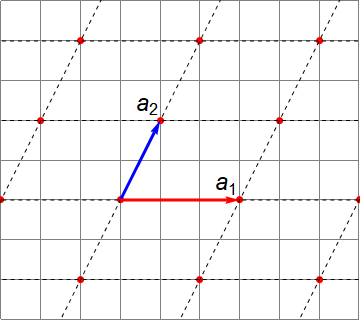
\includegraphics[width=1.0\textwidth]{HLBravaisLattice}
%            \end{center}\end{minipage}
%            \hspace{2ex}
%            \begin{minipage}[c]{0.46\textwidth}
%basis vectors \\ ${\bf a}_1=(3,0)$, ${\bf a}_2=(1,2)$
%            \end{minipage}
%\end{center}
%    \end{block}
%
%\vfill
%
%6 field values, on 6 lattice sites $z=(n,\zeit)$,
%$[3\!\times\!2]$ rectangle:
%\[
% \left[
% \begin{array}{ccc}
% \ssp_{01} & \ssp_{11} & \ssp_{21} \\
% \ssp_{00} & \ssp_{10} & \ssp_{20}
% \end{array}
% \right]
%\]
%\end{frame} %%%%%%%%%%%%%%%%%%%%%%%%%%%%%%%%%%%%%%%%%%%%%%
%

\begin{frame}{note : \catlatt\ dances over a parquet floor}
\begin{itemize}
  \item[(so far)]
latticization of spacetime continuum :\\
{\color{blue}\emph{field}} $\ssp(x,\zeit)$ over spacetime coordinates
$(x,\zeit)$\\ for {\color{blue}\emph{any}} field theory

~~~~~~~~~~~~~~~$\Rightarrow$

set of lattice site values $\ssp_z=\ssp(n\Delta{L},\zeit\Delta{T})$.\\
Subscript $z=(n,\zeit)\in\integers^d$ is a discrete $d$\dmn\
spacetime {\color{blue}\emph{coordinate}} over which the field $\ssp$ lives
\medskip

distinct spacetime tiles have tilted shapes
$\LTS{}{}{}$
\bigskip

  \item[(next)]
\catlatt\ {\color{blue}\emph{field}} $\ssp_{z}$ is confined to $[0,1)$\\
That imparts a $\integers^1$ lattice structure on {\fundPip} $\jMorb$
basis vectors ; fundamental fact then counts all periodic
{\color{blue}lattice \emph{states}} $\Xx_\Mm$ for \\
a given spacetime tile
$\LTS{}{}{}$
\end{itemize}
\end{frame} %%%%%%%%%%%%%%%%%%%%%%%%%%%%%%%%%%%%%%%%%%%%%%


\begin{frame}{fundamental fact works for a spacetime lattice (!)}

    \begin{block}{recall Bernoulli fundamental fact example ?}
\begin{center}
            \begin{minipage}[c]{0.32\textwidth}\begin{center}
% ChaosBook {fig:BernPartExam} % BernCyc2Jacob.svg
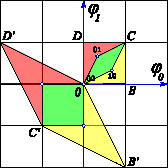
\includegraphics[width=1.0\textwidth]{BernCyc2JacobUnit}
            \end{center}\end{minipage}
            \hspace{2ex}
            \begin{minipage}[c]{0.46\textwidth}
unit hyper-cube $\Xx\in[0,1)^2$
\medskip

~~~~~~~~~~~~~~~~$\Rightarrow\jMorb\Rightarrow$
\medskip

{\fundPip}
            \end{minipage}
\end{center}
%$\jMorb\,[0BCD] =$ {\fundPip} $[0B'C'D']$
    \end{block}

\vfill

spacetime {\fundPip} basis
vectors $\jEigvec[j]$ \\
$=$ columns of the {\color{blue}\jacobianOrb}
\beq
\jMorb = (\jEigvec[1]|\jEigvec[2]|\cdots|\jEigvec[\speriod{}\period{}])
\ee{lattJac}
\end{frame} %%%%%%%%%%%%%%%%%%%%%%%%%%%%%%%%%%%%%%%%%%%%%%


%\begin{frame}{solving $1D$ cat map using Green's functions}
%\begin{block}{the Green's function $\Xx=g\,\Mm$ for a period \period{} solution of}
%\[
% (\Box -s+2)\ssp_{t} = \m_t
%%    \,, \qquad
%\] %\ee{LinearConn}
%
%\medskip
%\end{block}
%\begin{block}{is a Toeplitz matrix $\gd$ that satisfies}
%\bea
% (\D \gd)_{tt'}&=&\delta_{tt'}\,, \qquad t,t'\in 0,1,2,\cdots,\period{}-1
%% \label{1DGreenFun0} \ee{1DGreenFunDirichlet}
%        \continue
%   & &  \continue
%\D &=&\left(\begin{array}{ccccccc}
% s&-1 & 0 & 0 &\dots &0&-1 \\
%-1 &  s&-1 & 0 &\dots &0&0 \\
%0 &-1 &  s&-1 &\dots &0 & 0 \\
%\vdots & \vdots &\vdots & \vdots & \ddots &\vdots &\vdots\\
%0 & 0 & \dots &\dots &\dots  & s&-1 \\
%-1 & 0 & \dots &  \dots &\dots&-1 &  s
%        \end{array} \right )
%\nnu
%\eea %ee{3diagToeplitz}
%\medskip
%\end{block}
%\end{frame} %%%%%%%%%%%%%%%%%%%%%%%%%%%%%%%%%%%%%%%%%%%%%%

%\begin{frame}{
%the 3-letter translations alphabet \;+\; the Markov graph
%             }
%
%\medskip
%
%generates the admissible orbits of $1D$ cat map
%\[ %beq
%\Ssym{t}\in\{\underline{1},0,1\}
%\] %ee{threeLett}
%example : all admissible 4-cycles
%\bea
%{\bf x}_{0 0 1 \underline{1}} &=& \frac{1}{15}
%\left[
%\begin{array}{cccc}
% {-1} &
% {1} &
% {4} &
% {-4}
%\end{array}
%\right]
%    \,,\qquad
%{\bf x}_{0 1 0 \underline{1}}= \frac{1}{15}
%\left[
%\begin{array}{cccc}
% {0} &
% {5} &
% {0} &
% {-5}
%\end{array}
%\right]
%    \continue
%{\bf x}_{0 1 \underline{1}1} &=& \frac{1}{15}
%\left[
%\begin{array}{cccc}
% {4} &
% {6} &
% {-1} &
% {6}
%\end{array}
%\right]
%    \,,\qquad
%{\bf x}_{0 1 1 \underline{1}}= \frac{1}{15}
%\left[
%\begin{array}{cccc}
% {2} &
% {8} &
% {7} &
% {-2}
%\end{array}
%\right]
%    \continue
%% Predrag 2018-02-19 replaced the
%% old 6 \cycle{3125} \\  1 0 1 \underline{1} = 4 \cycle{1253}
%% by new No. 6:
%% 6 \cycle{1133} \\  0 0 1            1
%{\bf x}_{0 0 1 1} &=& \frac{1}{15}
%\left[
%\begin{array}{cccc}
% {5} &
% {5} &
% {10} &
% {10}
%\end{array}
%\right]
%    \,,\qquad
%{\bf x}_{1 1 1 \underline{1}}= \frac{1}{15}
%\left[
%\begin{array}{cccc}
% {9} &
% {11} &
% {9} &
% {1}
%\end{array}
%\right]
%    \continue
%{\bf x}_{1 1 1 0} &=& \frac{1}{15}
%\left[
%\begin{array}{cccc}
% {12} &
% {13} &
% {12} &
% {8}
%\end{array}
%\right]
%    \,,\qquad
%{\bf x}_{1 1 0 \underline{1}}= \frac{1}{15}
%\left[
%\begin{array}{cccc}
% {7} &
% {8} &
% {2} &
% {-2}
%\end{array}
%\right]
%    \continue
%{\bf x}_{0 0 \underline{1}1} &=& \frac{1}{15}
%\left[
%\begin{array}{cccc}
% {1} &
% {-1} &
% {-4} &
% {4}
%\end{array}
%\right]
%\label{4cyclesPerPoints}
%\eea
%\end{frame} %%%%%%%%%%%%%%%%%%%%%%%%%%%%%%%%%%%%%%%%%%%%%%

\begin{frame}{example : spacetime periodic $\BravCell{3}{2}{0}$
              lattice state}
\[
F[\Xx] = \jMorb\Xx+\Mm = 0
\]
6 field values, on 6 lattice sites $z=(n,\zeit)$,
$\BravCell{3}{2}{0}$ tile :
\[
\Xx_{\BravCell{3}{2}{0}} =
 \left[
 \begin{array}{ccc}
 \ssp_{01} & \ssp_{11} & \ssp_{21} \\
 \ssp_{00} & \ssp_{10} & \ssp_{20}
 \end{array}
 \right]
\,,\qquad %\Leftrightarrow\qquad
6\,\Mm_{\BravCell{3}{2}{0}} =
%%%%%%%%%%%%%%%%%%%%%%%%%%%%%%%%%%%%%%%%%%%%%%%%%%%%%%%%%%%%%
% HL 2020-06-09 siminos/figSrc/han/Mathematica/ColorBlock.nb
            \begin{minipage}[c]{0.15\textwidth}\begin{center}
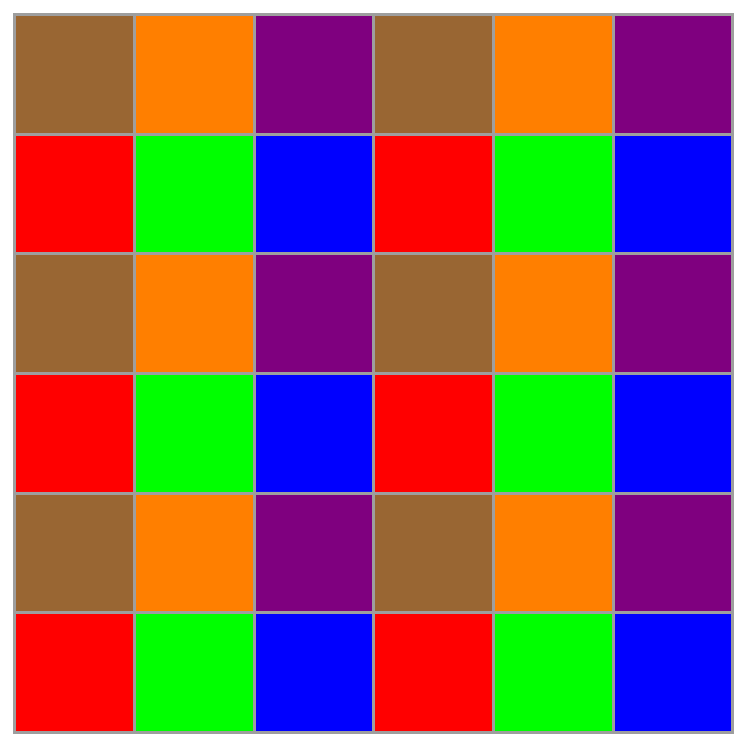
\includegraphics[width=1.0\textwidth]{HL320Block} %\\$\BravCell{3}{2}{0}$ %(b)
            \end{center}\end{minipage}
\]
where the region of symbol plane shown is tiled by 6 repeats of the
$\Mm_{\BravCell{3}{2}{0}}$ \brick, and tile {\color{green}color} = value of
symbol $\Ssym{z}$
\medskip

`stack up' vectors and matrices, vectors as 1\dmn\ arrays,
\beq
\Xx_{\BravCell{3}{2}{0}} =
\left(\begin{array}{c}
 \ssp_{01} \\
 \ssp_{00} \\
  \hline
 \ssp_{11} \\
 \ssp_{10} \\
  \hline
 \ssp_{21} \\
 \ssp_{20} \\
      \end{array}\right)
\,,\qquad
\Mm_{\BravCell{3}{2}{0}} =
\left(\begin{array}{c}
 \Ssym{01} \\
 \Ssym{00} \\
  \hline
 \Ssym{11} \\
 \Ssym{10} \\
  \hline
 \Ssym{21} \\
 \Ssym{20} \\
        \end{array}\right)
\ee{3times2blockVect}
\end{frame} %%%%%%%%%%%%%%%%%%%%%%%%%%%%%%%%%%%%%%%%%%%%%%

\begin{frame}{}
with the $[6\!\times\!6]$ {\jacobianOrb} in block-matrix form
\beq
\jMorb_{\BravCell{3}{2}{0}} =
\left(
\begin{array}{cc|cc|cc}
 -2 s & 2 & 1 & 0 & 1 & 0  \\
 2 & -2 s & 0 & 1 & 0 & 1  \\
  \hline
 1 & 0 & -2 s & 2 & 1 & 0  \\
 0 & 1 & 2 & -2 s & 0 & 1  \\
  \hline
 1 & 0 & 1 & 0 & -2 s & 2  \\
 0 & 1 & 0 & 1 & 2 & -2 s
\end{array}
\right)
\ee{3times2basisVecs}
\end{frame} %%%%%%%%%%%%%%%%%%%%%%%%%%%%%%%%%%%%%%%%%%%%%%

\begin{frame}{}

{\fundPip} basis
vectors $\jEigvec[j]$ are
the columns of the {\jacobianOrb}
\beq
\jMorb_{\BravCell{3}{2}{0}} =
\left(
\begin{array}{c|c|c|c|c|c}
 -2 s & 2 & 1 & 0 & 1 & 0  \\
 2 & -2 s & 0 & 1 & 0 & 1  \\
 1 & 0 & -2 s & 2 & 1 & 0  \\
 0 & 1 & 2 & -2 s & 0 & 1  \\
 1 & 0 & 1 & 0 & -2 s & 2  \\
 0 & 1 & 0 & 1 & 2 & -2 s
\end{array}
\right)
\ee{3times2basisVecs}
the `fundamental fact' now yields the number of
solutions for any half-integer ${s}$ as {\color{blue}\HillDet}
\beq
N_{\BravCell{3}{2}{0}} = |\Det\jMorb_{\BravCell{3}{2}{0}}|
                   = 4({s}-2)s(2{s}-1)^2 (2{s}+3)^2
\ee{N3times2}
\end{frame} %%%%%%%%%%%%%%%%%%%%%%%%%%%%%%%%%%%%%%%%%%%%%%

\begin{frame}{can count \catlatt\ states for any $\Lambda=\LTS{}{}{}$}
\begin{center}
{\scriptsize
\begin{tabular}{lllr}
\\[-16pt]
$~~~\Lambda$
                         & ~~~$N_\Lambda(s)$ & $M_\Lambda(s)$
                                                 &$R$  \\
\hline
$\BravCell{1}{1}{0}$    &   $2({s}-2)$ & $2({s}-2)$ & 1 \\
$\BravCell{2}{1}{0}$    &   $2({s}-2)2s$ & $2({s}-2)\frac{1}{2}(2{s}-1)$   & 2 \\
$\BravCell{2}{1}{1}$  &   $2({s}-2)2({s}+2)$ & $2({s}-2)\frac{1}{2}(2{s}+3)$  & \\
$\BravCell{3}{1}{0}$    &   $2({s}-2)(2{s}-1)^2$ & $2({s}-2)\frac{4}{3}({s}-1){s}$ &  \\
$\BravCell{3}{1}{1}$  &   $2({s}-2)4({s}+1)^2$ & $2({s}-2)\frac{1}{3}(2{s}+1)(2{s}+3)$ & \\
%was $2({s}-2)(2{s}-1)^2$
%$\BravCell{3}{1}{2}$  &   $2({s}-2)4({s}+1)^2$ & $2({s}-2)\frac{1}{3}(2{s}+1)(2{s}+3)$ & \\
%was $2({s}-2)(2{s}-1)^2$
$\BravCell{4}{1}{0}$    &   $2({s}-2)8({s}-1)^2{s}$ & $2({s}-2)\frac{1}{2}(2{s}-3)(2{s}-1)s$ & \\
$\BravCell{4}{1}{1}$  &   $2({s}-2)8s^2({s}+2)$ & $2({s}-2)\frac{1}{2}({s}+2)(2{s}-1)(2{s}+1)$ & \\
%was $2({s}-2)8({s}-1)^2{s}$
$\BravCell{4}{1}{2}$  &   $2({s}-2)8({s}+1)^2{s}$ & $2({s}-2)\frac{1}{2}(2{s}+3)(2{s}+1)s$     & \\
%was $2({s}-2)8({s}-1)^2{s}$
$\BravCell{4}{1}{3}$  &   $2({s}-2)8s^2({s}+2)$ & $2({s}-2)\frac{1}{2}({s}+2)(2{s}-1)(2{s}+1)$ &  \\
%was $2({s}-2)8({s}-1)^2{s}$
$\BravCell{5}{1}{0}$    & $2({s}-2)\left(4{s}^2-6{s}+1\right)^2$ & $2({s}-2)\frac{4}{5}({s}-1)(2{s}-3)(2{s}-1)s$
                                  & \\
$\BravCell{5}{1}{1}$  & $2({s}-2)16\left({s}^2+{s}-1\right)^2$ & $2({s}-2)\frac{1}{5}(2{s}-1)(2{s}+3)(4{s}^2+4{s}-5)$
                                  & \\
%was $2({s}-2)\left(4{s}^2-6{s}+1\right)^2$
$\BravCell{2}{2}{0}$    & $2({s}-2)8s^2({s}+2)$ & $2({s}-2)\frac{1}{2}(2{s}-1)(2{s}^2+5{s}+1)$  & 1 \\
$\BravCell{2}{2}{1}$  & $2(s-2)8s (s+1)^2$ & $2({s}-2)\frac{1}{2}(2{s}+1)(2{s}+3)s$ &  \\
%was $2(s-2)8s^2 (s+2)$
$\BravCell{3}{2}{0}$    & $2({s}-2)2s(2{s}-1)^2 (2{s}+3)^2$
	& $2({s}-2)\frac{2}{3}(2{s}-1)(4{s}^3+10{s}^2+3{s}-5)s$
                                  &  \\
$\BravCell{3}{2}{1}$  & $2({s}-2)32{s}^3({s}+1)^2$
	& $2 ({s}-2) \frac{1}{6} (2 {s}-1) (2 {s}+1) (8 {s}^3+16 {s}^2+10 {s}+3)$
                                  &  \\
%$\BravCell{3}{2}{2}$  & $2({s}-2)32{s}^3 ({s}+1)^2$
%	& $2 ({s}-2) \frac{1}{6} (2 {s}-1) (2 {s}+1) (8 {s}^3+16 {s}^2+10 {s}+3)$
%                                  &  \\
$\BravCell{3}{3}{0}$    & $2({s}-2)16({s}+1)^4(2{s}-1)^4$
                                  &  \\
%$\BravCell{3}{3}{1}$  & $2({s}-2)(2{s}-1)^2(8{s}^3+12{s}^2-1)^2$
%	            &  \\
%$\BravCell{3}{3}{2}$  & $2({s}-2)(2{s}-1)^2(8{s}^3+12{s}^2-1)^2$
%                &
\end{tabular}
} %end \scriptsize
\end{center}
\end{frame} %%%%%%%%%%%%%%%%%%%%%%%%%%%%%%%%%%%%%%%%%%%%%%

\begin{frame}{we can count !}

\begin{enumerate}
  \item can construct all spacetime tilings,
  from small tiles to as large as you wish
  \item for each spacetime tile $\LTS{}{}{}$,
can evaluate
$\sharp$ of doubly-periodic {\color{blue}lattice states} for a tile
\[
N_{\LTS{}{}{}}
\]
  \item
$\sharp$ {\color{blue}prime orbits} for a tile
\[
M_{\LTS{}{}{}}
\]
\end{enumerate}
\end{frame} %%%%%%%%%%%%%%%%%%%%%%%%%%%%%%%%%%%%%%%%%%%%%%

\begin{frame}{zeta function for a field theory ???} % much like Ising model}
% Ihara zeta functions ?
\begin{block}{`\po s' are now \twots\ (tiles)}
each a spacetime lattice tile  $p$ of area $A_p = L_p T_p$\\
that cover the \statesp\ with `natural weight'
\[
% Z(s) \approx
\sum_{p} \frac{1}                       % e^{-A_p s}}
              {\left|\Det\jMorb_p\right|}
\]
\end{block}
%\begin{block}{symbolic dynamics : $d$\dmn}
%essential to encode shadowing
%\end{block}

\vfill
at this time :
\begin{itemize}
\item $d=1$ temporal cat zeta function works like charm
\item $d=2$ {\catlatt} works, order by order
\item $d\geq2$ Navier-Stokes  zeta is still but a dream
\end{itemize}
\end{frame} %%%%%%%%%%%%%%%%%%%%%%%%%%%%%%%%%%%%%%%%%%%%%%

\begin{frame}{\catlatt\ \tzeta}
know how to evaluate the number of doubly-periodic lattice states
\[
N_{\LTS{}{}{}}
\,,
\]
for a given
$\LTS{}{}{}$
finite spacetime tile
\bigskip

now substitute these numbers of lattice states into the
{topological} zeta func\-tion
\bea
\zetatop(z_1,z_2)
 &=&
1 - \frac{{\mu}^2}
{z_1 + z_2 - 4 + z_1^{-1} + z_2^{-1}}
\qquad \mbox{\textcolor{red}{\Huge ??}}
\eea
but that's just a guess - we currently have no generating function that
presents all solutions in a compact form
\bigskip


\vfill
{\Huge \textcolor{red}{funky... \hfill not solved :(}}
\end{frame} %%%%%%%%%%%%%%%%%%%%%%%%%%%%%%%%%%%%%%%%%%%%%%

\begin{frame}{Zetastan : lost in translation}
\begin{center}
\hfill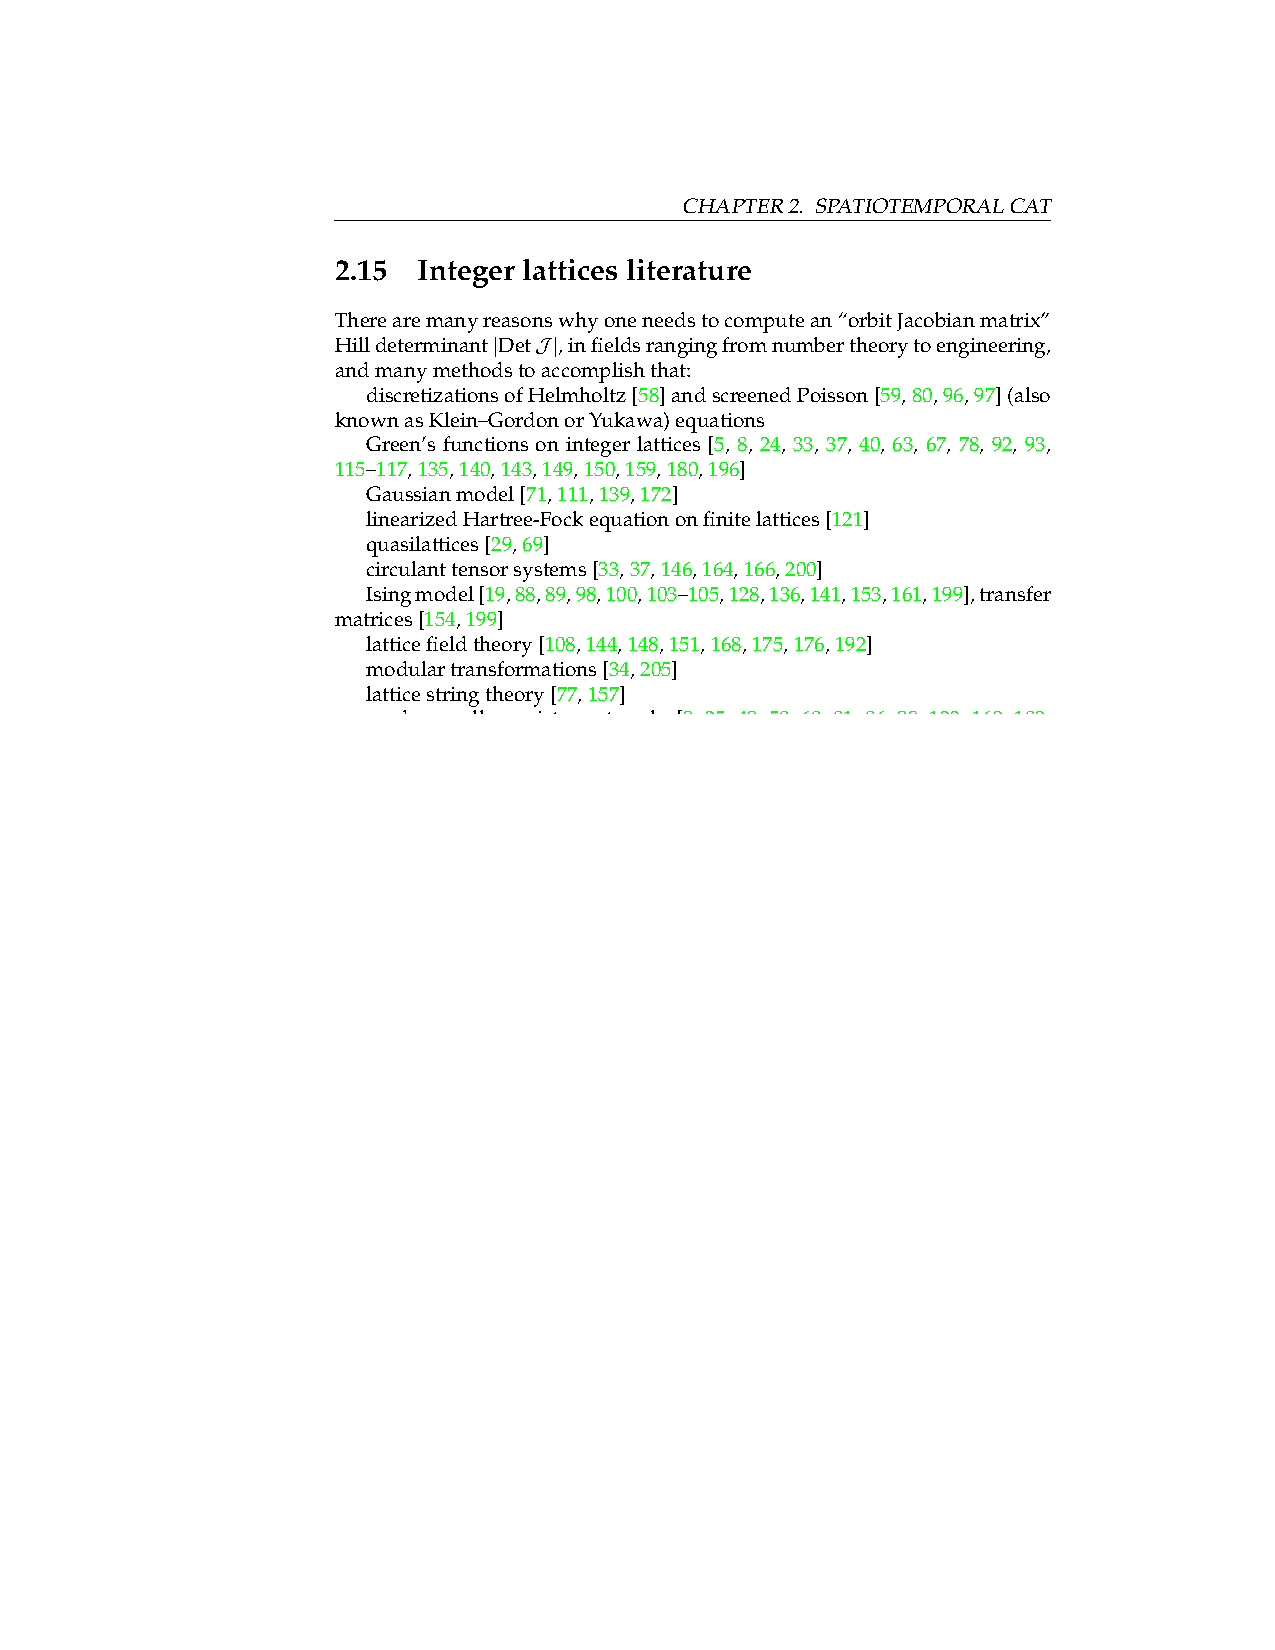
\includegraphics[width=0.90\textwidth]{lattLitClip1}
\end{center}
\end{frame} %%%%%%%%%%%%%%%%%%%%%%%%%%%%%%%%%%%%%%%%%%%%%%

\begin{frame}{Zetastan : lost, but not alone}
\begin{center}
\hfill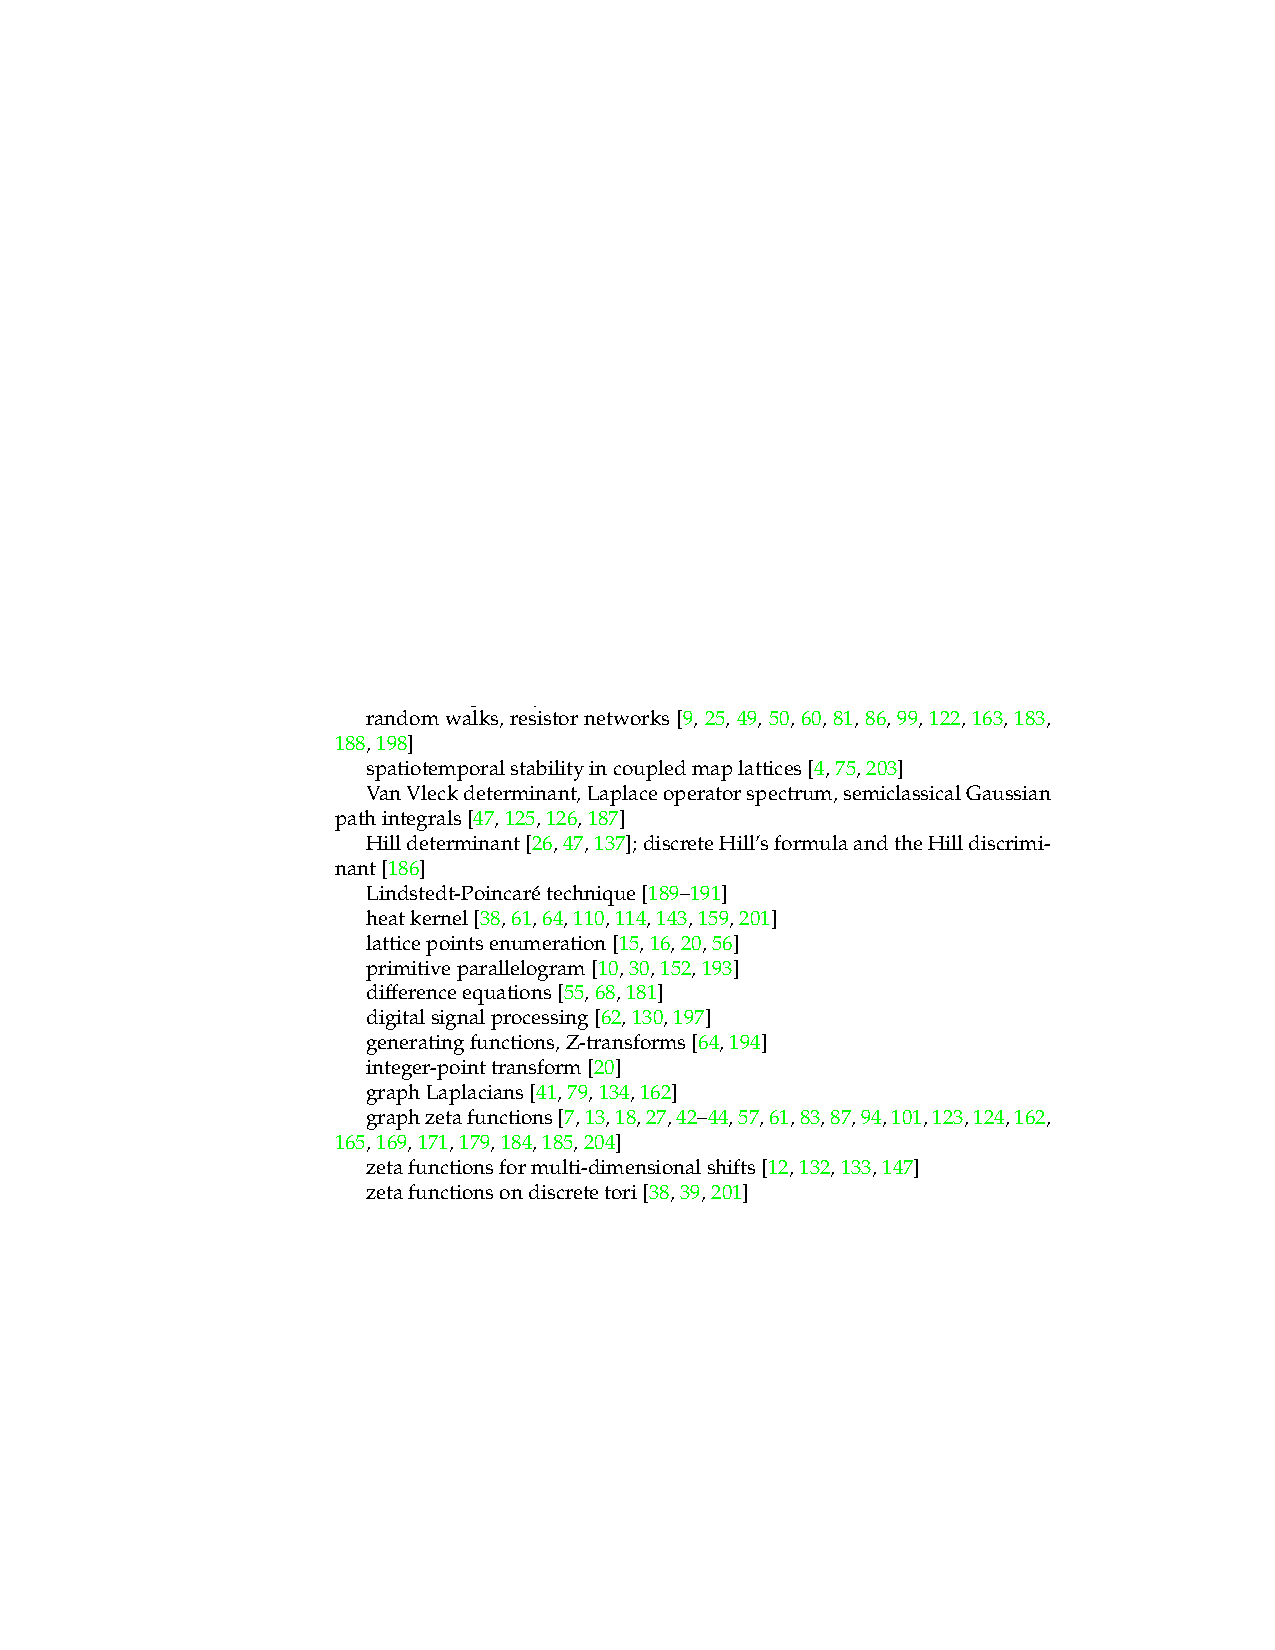
\includegraphics[width=0.90\textwidth]{lattLitClip2}
\end{center}
\end{frame} %%%%%%%%%%%%%%%%%%%%%%%%%%%%%%%%%%%%%%%%%%%%%%

\begin{frame}{side remark to experts}
    \begin{block}{SL$_2(\integers)$ unimodular invariance of square lattice}
\begin{center}
  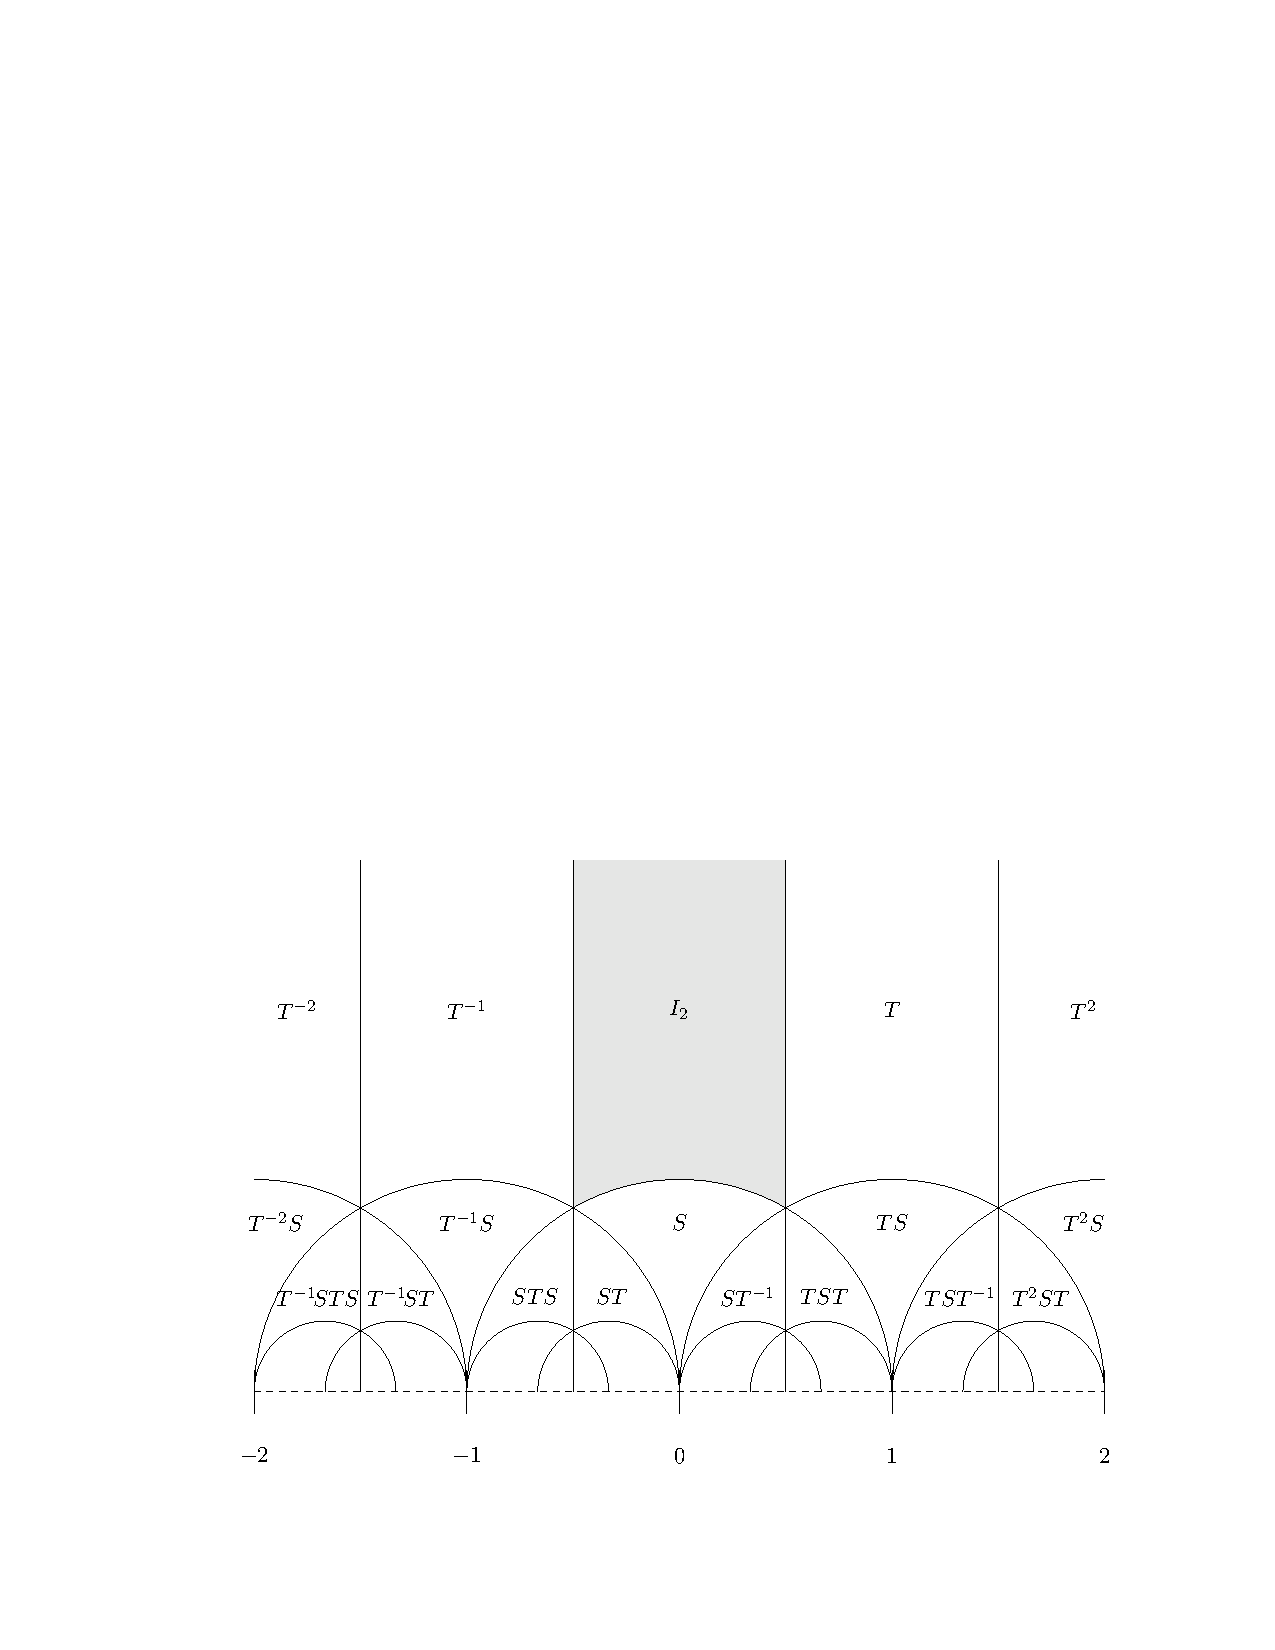
\includegraphics[width=0.65\textwidth]{ConradSL2Z}
\end{center}
Action on the complex upper half-plane by linear
fractional transformations $T$ and $S$.
~~~~~(figure: Keith Conrad)
    \end{block}
\bigskip

infinitely many `Bravais cells' for the same lattice
\end{frame} %%%%%%%%%%%%%%%%%%%%%%%%%%%%%%%%%%%%%%%%%%%%%%

\begin{frame}{but, is this}
\vfill
\begin{center}
{\huge chaos?}
\end{center}
\vfill
yes, short tiles are exponentially good `shadows' of the larger ones,
so can attain any desired accuracy
\end{frame} %%%%%%%%%%%%%%%%%%%%%%%%%%%%%%%%%%%%%%%%%%%%%%

\begin{frame}{is \catlatt\ `chaotic'?}
in time-evolving deterministic chaos any chaotic trajectory is
{\color{blue}shadowed by shorter \po s}
\bigskip

in \spt\ chaos, any unstable lattice state is {\color{blue}shadowed by
smaller \twots}
(Gutkin \etal\footfullcite{GutOsi15}${}^{,}${}\footfullcite{GHJSC16})

\vfill

next figure : code the \Mm\ symbol \brick\  $\ssp_{n\zeit}$ at the
lattice site $n\zeit$ with (color) alphabet
\[
\Ssym{t\ell} \in \A=\{\underline{1},0,1,2,\cdots\}=
\{%
{\color{red}red},
{\color{green}green},
{\color{blue}blue},
{\color{yellow}yellow},\cdots%
\}
\]

\end{frame} %%%%%%%%%%%%%%%%%%%%%%%%%%%%%%%%%%%%%%%%%%%%%%

\begin{frame}{shadowing, symbolic dynamics space}
\begin{center}
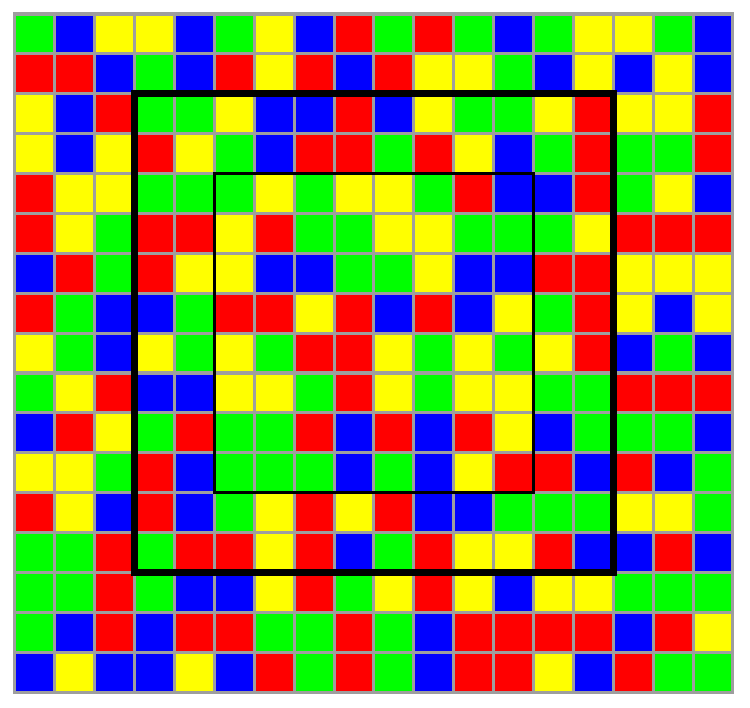
\includegraphics[width=0.45\textwidth]
{AKSs7colrBorderM1}\hspace{0.7cm}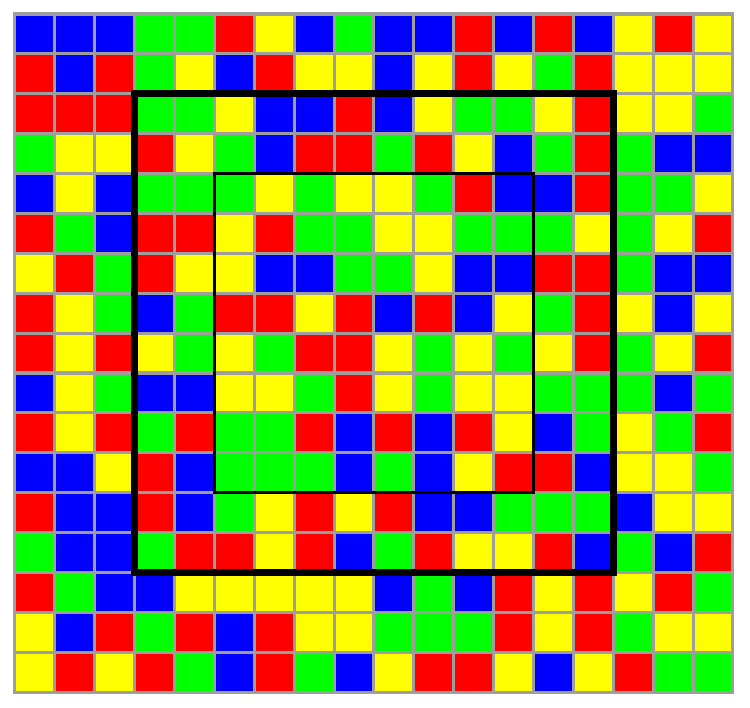
\includegraphics[width=0.45\textwidth]
{AKSs7colrBorderM2}
\end{center}
2d symbolic representation $\Mm_j$ of two lattice states $\Xx_j$
shadowing each other within the shared
\brick\ $\Mm_{\R}$ %=\Mm_{\R_{0}} \cup \Mm_{\R_{1}}$ (blue)

\begin{itemize}
  \item border $\R$ (thick black) %, interior $\R_{0}$ (thin black)
  \item symbols outside \R\ differ
\end{itemize}
\vfill
$s=7/2$    \hfill                          Adrien Saremi 2017
%\label{fig:AKScloseActSymb}
%%%%%%%%%%%%%%%%%%%%%%%%%%%%%%%%%%%%%%%%%%%%%%%%%%%%%%%%%%%%%%%%%%%%%%%
\end{frame} %%%%%%%%%%%%%%%%%%%%%%%%%%%%%%%%%%%%%%%%%%%%%%

\begin{frame}{shadowing} %, \statesp}
%%%%%%%%%blogCats \label{fig:AKSs7dist} %%%%%%%%%%%%%%%%%%%%%%%%%%%%%
\begin{center}
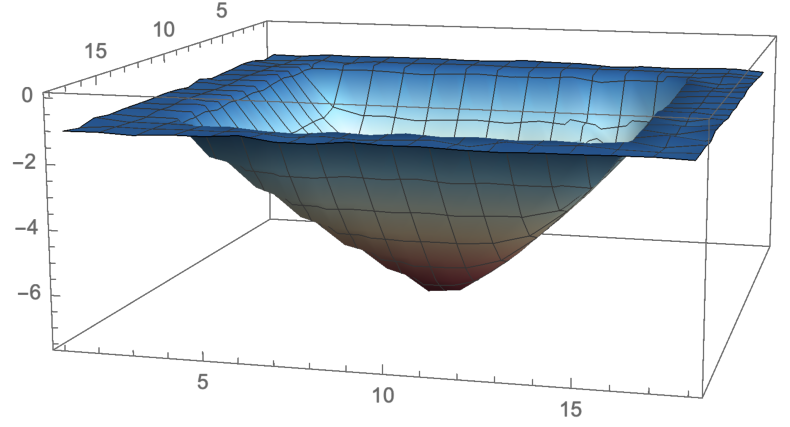
\includegraphics[width=0.65\textwidth]
{HL18ShadowingDistanceAverageLog3D}
\end{center}

\bigskip

the logarithm of the average of the absolute value of site-wise distance
\[
\ln|\ssp_{2,z}-\ssp_{1,z}|
\]
averaged over 250 solution pairs
\medskip

note the exponential falloff of the distance away from the center of the
shared \brick\ $\R$ %=\R_{0} \cup \R_{1}$.
\medskip

$\Rightarrow$ within the interior of the shared \brick,

\hfill \textcolor{blue}{shadowing is exponentially close}
\end{frame} %%%%%%%%%%%%%%%%%%%%%%%%%%%%%%%%%%%%%%%%%%%%%%

\begin{frame}{take-home :   }
\begin{center}
            \begin{minipage}[c]{0.40\textwidth}\begin{center}
{\color{purple}harmonic} field theory
\bigskip

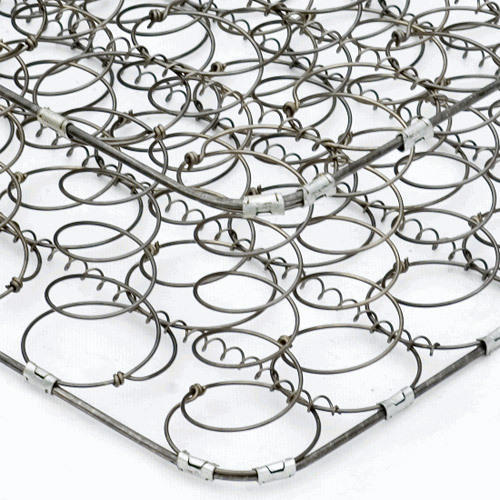
\includegraphics[width=0.85\textwidth]{mattressSpring}\\
{\color{blue}tight-binding} model \\ ({\color{blue}Helmholtz})
            \end{center}\end{minipage}
            \hspace{2ex}
            \begin{minipage}[c]{0.46\textwidth}\begin{center}
{\color{purple}chaotic} field theory\\
\bigskip
\bigskip
\bigskip

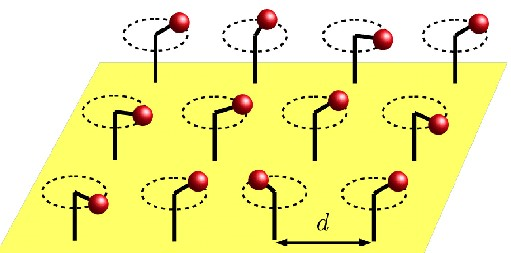
\includegraphics[width=1.0\textwidth]{flagellum1}\\
\bigskip

Euclidean {\color{blue}Klein-Gordon} \\ (damped {\color{blue}Poisson})
            \end{center}\end{minipage}
\end{center}
\end{frame}%%%%%%%%%%%%%%%%%%%%%%%%%%%%%%%%%%%%%%%%%%%%%%

\begin{frame}{our song of chaos has been sang. what next ?}
\begin{enumerate}
              \item \textcolor{gray}{\small
%what this is about
%              \item
coin toss
              \item
kicked rotor
              \item
\catlatt
                  }
              \item {\Large
bye bye, dynamics
%                  }\textcolor{gray}{\small
%              \item
%bye bye, dynamics
                    }
            \end{enumerate}
\end{frame} %%%%%%%%%%%%%%%%%%%%%%%%%%%%%%%%%%%%%%%%%%%%%%



\end{document}
